%==================================================
%      PREAMBOLO e DICHIARAZIONI INIZIALI
%==================================================
\documentclass[10pt,oneside,a4paper]{article}

\usepackage[latin1]{inputenc} 
\usepackage[italian]{babel}
\usepackage[T1]{fontenc}
\usepackage{siunitx} %Inserisce automaticamente i dati con le unit�  di misura correttamente formattate del SI (utilizzo: \SI{0.82}{m^2}, in generale \SI{misura con il punto decimale}{unit�  di misura})
\sisetup{output-decimal-marker = {.}, separate-uncertainty = true, input-uncertainty-signs = \pm, detect-weight=true, detect-family=true} %per usare SI con il punto decimale
\usepackage{listings} %Per citare codice informatico formattandolo correttamente
\usepackage{amsmath,amsthm,verbatim,amssymb,amsfonts,amscd,graphicx,mathtools}
\usepackage[makeroom]{cancel}
\newcommand{\abs}[1]{\left\lvert\,#1\,\right\rvert}
\usepackage{geometry}
\usepackage{epigraph}
\usepackage{booktabs}	%tabelle migliorate
\usepackage{tablefootnote}	%note a pi� di pagina in tabella
\usepackage{threeparttable} %tabella con note a pi� di tabella
\usepackage{caption}	%descrizione per figure
\usepackage{dblfnote}
\captionsetup{tableposition=top,figureposition=bottom,font=small} %setup descrizione
\usepackage{float}
\usepackage{esvect} %vettori
\usepackage{longtable} %tabelle lunghe
\usepackage[dvipsnames]{xcolor}
\definecolor{sepia}{HTML}{80002A}
\usepackage[colorlinks=true, citecolor=black, linkcolor=sepia, urlcolor=black]{hyperref}
\usepackage{mathrsfs}
\usepackage{circuitikz}
\ctikzset{bipoles/resistor/height=0.2}
\ctikzset{bipoles/resistor/width=0.4}
\ctikzset{tripoles/american nand port/height=0.7}
\ctikzset{tripoles/american nand port/width=0.8}
\usepackage{enumitem} %Liste senza spazi verticali
\setlist{noitemsep}
\usepackage{amsmath}

\interfootnotelinepenalty=10000


\usepackage{multicol}
\newenvironment{Figure}
  {\par\medskip\noindent\minipage{\linewidth}}
  {\endminipage\par\medskip}

\newcommand{\var}{\operatorname{var}}
\newcommand{\cov}{\operatorname{cov}}


\usepackage{listings} %Per inserire codice
\lstnewenvironment{codice_c}[1][]
{\lstset{basicstyle=\small\ttfamily, columns=fullflexible,
keywordstyle=\color{red}\bfseries, commentstyle=\color{blue},
language=C, basicstyle=\small,
numbers=left, numberstyle=\tiny,
stepnumber=2, numbersep=5pt, frame=shadowbox,  showstringspaces=false, #1}}{}

%==================================================
%                  PRIMA PAGINA
%==================================================

\title{\textsc{\textbf{Esercitazione 6}: Elettronica Digitale, Porte Logiche}}
\author{\small{G. Galbato Muscio} \and \small{L. Gravina} \and \small{L. Graziotto}}
\date{27 Novembre 2018}

\begin{document}
	\begin{figure}
		\centering
		
\includegraphics[scale=0.5, trim={2.8cm 8.9cm 0 9cm}, clip]{logo.png}
	\end{figure}
	\maketitle
	\begin{center} 
		\fbox{{\fontsize{12pt}{8mm}\textsc{Gruppo 11}}} \\
	\end{center}
\hrule
\vspace{0.5cm}
\renewcommand{\abstractname}{Abstract}
\begin{abstract}
Si studiano i livelli di commutazione delle porte logiche TTL dell'integrato 74LS00. Si realizza un circuito XOR con porte NAND e un multiplexer a due ingressi. Si costruisce un flip-flop set-reset con porte NAND.
\end{abstract}
\vspace{4cm}
\tableofcontents %Indice
\newpage


\pagebreak
\begin{multicols}{2}
%==================================================
%             LIVELLI COMMUTAZIONE TTL
%==================================================
\section{Livello di commutazione delle porte logiche TTL}
Si utilizzer� per tutta l'esperienza l'integrato 74LS00, che � alimentato con una tensione di \SI{5}{V}, mentre il \texttt{GND} � posto a massa, comune ai generatori di tensione e di segnali e all'oscilloscopio. Per visualizzare rapidamente il livello delle uscite saranno utilizzati dei LED, protetti da resistenze dell'ordine di \SI{500}{\ohm} verso massa. Inoltre, per realizzare gli ingressi statici si utilizza una resistenza di pull-up di \SI{0.997 \pm 0.005}{\kilo\ohm} connessa a \SI{5}{V}: questa resistenza � fondamentale sia per poter usare un interruttore verso massa collegato all'ingresso e dunque velocizzare la commutazione degli stati logici (senza questa resistenza ad interruttore chiuso si creerebbe un corto circuito del generatore verso massa), sia perch� in sua assenza il circuito costruito con l'integrato pu� perturbare in maniera non facilmente prevedibile il segnale in ingresso\footnote{Ad esempio, usando il generatore per inviare un'onda quadra in ingresso ad un multiplexer, senza la resistenza di pull-up il segnale generato verrebbe distorto fortemente, come verificabile sperimentalmente.}.

Si studia il livello di commutazione di una porta NOT realizzata utilizzando una porta NAND dell'integrato, mandando ad entrambi gli ingressi la stessa tensione $V_i$, compresa tra \SI{0}{} e \SI{5}{V} mediante un alimentatore diverso da quello utilizzato per alimentare l'integrato. Al variare della tensione $V_i$ si studia il conseguente andamento della tensione di uscita $V_o$, evidenziando i valori per cui si ha il passaggio dal livello logico $0$ a $1$ o viceversa. Il circuito � il seguente.

%\begin{circuitikz}
%\draw (0,0) node[ground]{} to[battery2=$V_i$, invert] (0,1.2) 
%(3,1.2) node[american nand port] (nand) {}
%(nand.in 1) to[short] (nand.in 2)  
%(nand.in 1 |- nand.out) to [short,-] (0,1.2)
%(nand.out) to[short, -*] ++(0.5,0) node[right]{$V_o$}
%;\end{circuitikz}

Si riportano in Tabella~\ref{tab:commutazione} i punti sperimentali individuati, e nel grafico di Figura~\ref{fig:commutazione} l'andamento della tensione in uscita in funzione della tensione di ingresso: il grafico � in scala semilog per poter apprezzare meglio la curva di discesa alle basse frequenze. Si osserva che il valore logico $1$ dell'uscita corrisponde ad una tensione di \SI{3.71 \pm 0.06}{V}, ottenuta dalla media dei primi $7$ punti, per i quali $V_o$ � costante all'aumentare di $V_i$, prima di raggiungere la regione in cui si ha la rapida decrescita. Allo stesso modo, prendendo la media degli ultimi $10$ punti, successivi alla regione di decrescita e nella zona di costanza di $V_o$, si ottiene per il valore logico $0$ una tensione corrispondente di \SI{58.8 \pm 0.3}{mV}.

Si confrontano i risultati ottenuti con le definizioni dello standard logico TTL, per le quali si ha un valore di $0$ logico (nel caso analizzato corrispondente all'$1$ in uscita dalla porta NOT) per una tensione di \SI{0.2}{V}, e un valore di $1$ logico (nel caso analizzato corrispondente allo $0$ in uscita dalla porta NOT) per una tensione di \SI{5}{V}. I valori misurati risultano lontani dallo standard TTL ideale, ma risultano invece compatibili con i valori riportati sul \emph{datasheet} dell'integrato \cite{WEBSITE:1}.



\begin{Figure}
	\begin{center}
	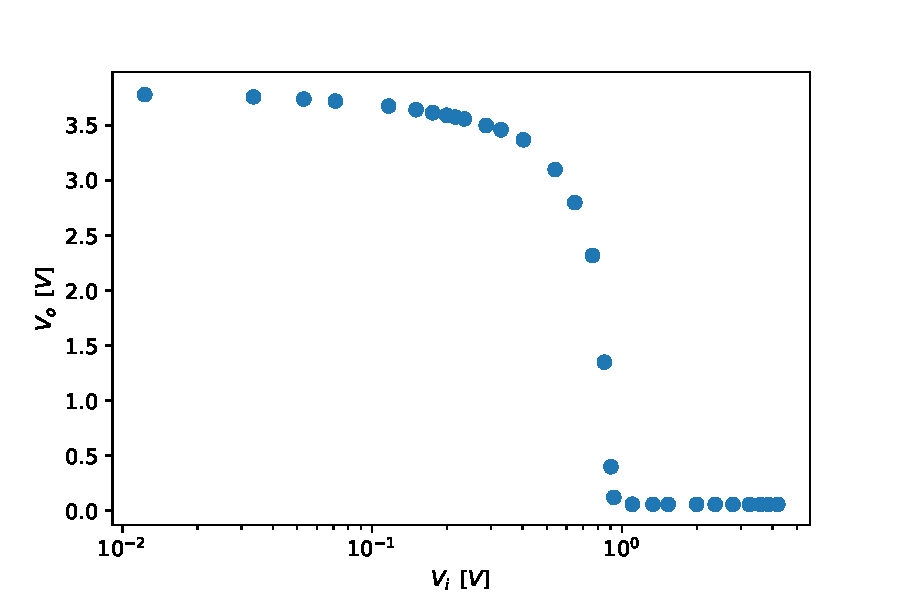
\includegraphics[width=\linewidth]{andamentoNAND.pdf}
	\captionof{figure}{Andamento di $V_o$ in funzione di $V_i$ per il NOT costruito con la porta NAND, scala semilog}
	\label{fig:commutazione}
	\end{center}
\end{Figure}

Per controllare se la transizione dipende dal valore di partenza, si costruisce un ciclo di \emph{isteresi}, ovvero si pone $V_i = \SI{0}{V}$, la si aumenta fino a \SI{5}{V} e si ritorna a \SI{0}{V}. Si riporta in Figura~\ref{fig:isteresi} il grafico per il ciclo.

\begin{Figure}
	\begin{center}
	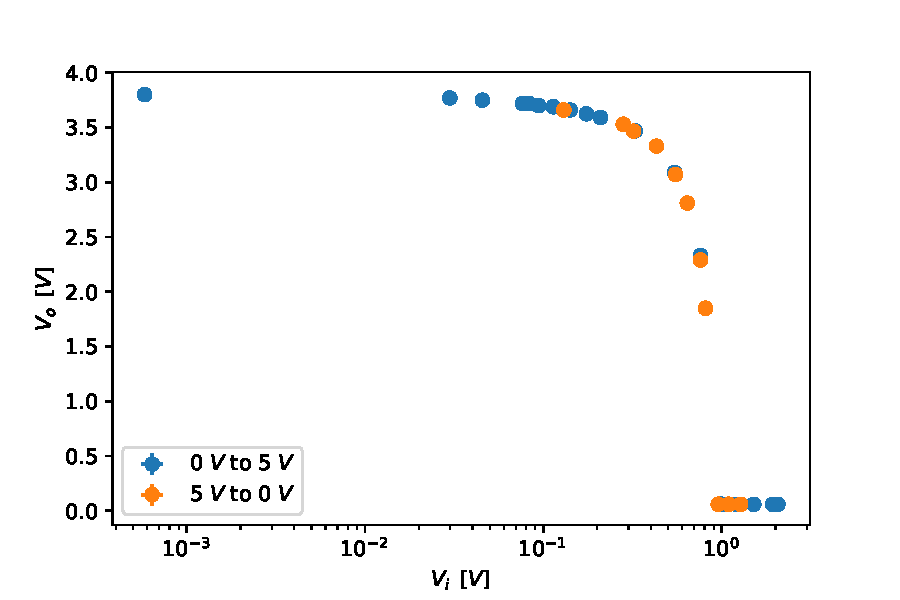
\includegraphics[width=\linewidth]{isteresi.pdf}
	\captionof{figure}{Cicli di \emph{isteresi} per la verifica dei livelli di commutazione della logica TTL, scala semilog}
	\label{fig:isteresi}
	\end{center}
\end{Figure}

Risulta evidente che le porte NAND dell'integrato non hanno memoria: il ciclo di isteresi risulta completamente analogo all'andamento riportato in Figura \ref{fig:triangolare}, inoltre non si riscontrano differenze tra le misure a tensione crescente e quelle a tensione decrescente.

Per vedere la curva caratteristica della porta NAND integralmente e in maniera pi� immediata, si pu� mandare al suo ingresso un'onda triangolare che oscilli tra $0$ e $\SI{5}{\volt}$ e visualizzare il segnale d'uscita su un oscilloscopio, come riportato in Figura \ref{fig:triangolare}. Questa curva risulta compatibile con le misure fatte, che per chiarezza del confronto sono riportate fino alla ventiduesima in scala lineare in Figura \ref{fig:commutazioneLin}.

\begin{Figure}
	\begin{center}
	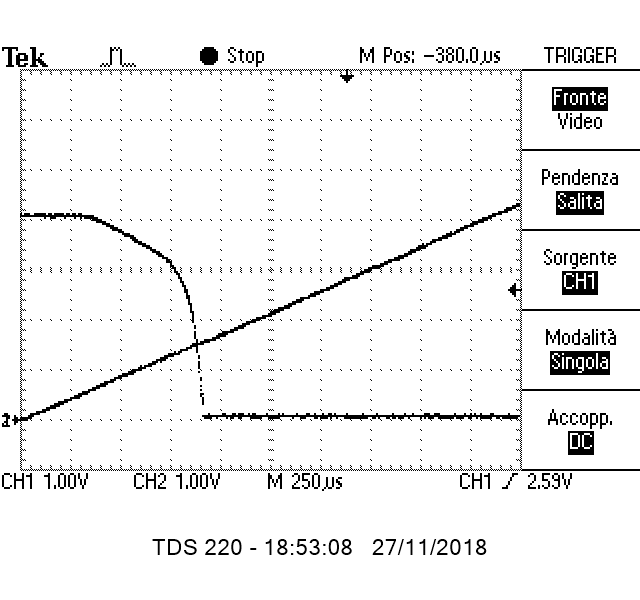
\includegraphics[width=\linewidth]{triangolareNAND.png}
	\captionof{figure}{Istantanea dell'oscilloscopio per visualizzare la curva caratteristica di un circuito XOR mandando in ingresso un'onda triangolare}
	\label{fig:triangolare}
	\end{center}
\end{Figure}

\begin{Figure}
	\begin{center}
	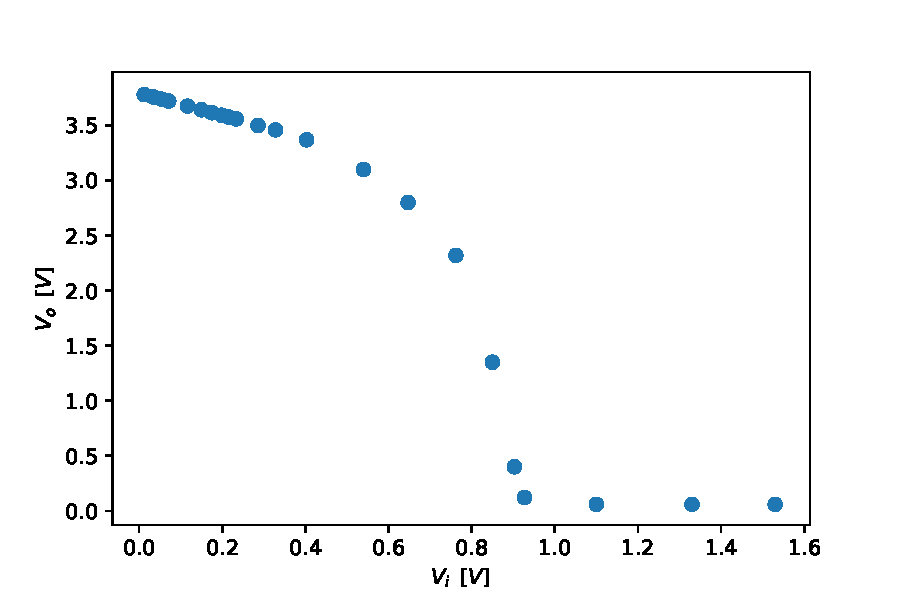
\includegraphics[width=\linewidth]{andamentoNANDlin.pdf}
	\captionof{figure}{Prime ventidue misure dell'andamento di $V_o$ in funzione di $V_i$ per il NOT costruito con la porta NAND, scala lineare}
	\label{fig:commutazioneLin}
	\end{center}
\end{Figure}

%==================================================
%             XOR CON PORTE NAND
%==================================================
\section{Circuito XOR con porte NAND}
Si costruisce un circuito XOR utilizzando le quattro porte NAND dell'integrato, realizzando la funzione logica:
\[
\begin{aligned}
Q &= \overline{\overline{A\left(\overline{AB}\right)}\cdot \overline{B\left(\overline{AB}\right)}} \\
&= \big(\overline{A}B\big) + \big(A \overline{B}\big),
\end{aligned}
\]
dove l'uguaglianza si ottiene applicando le Leggi di De Morgan. Il circuito � il seguente,

%\begin{circuitikz}
%\draw (0,0) node[american nand port] (nand1) {}
%(1.7,1) node[american nand port] (nand2) {}
%(1.7,-1) node[american nand port] (nand3) {}
%(3.4,0) node[american nand port] (nand4) {}
%(nand1.in 1) to[short, *-] ++(-0.5,0) node[left] {$A$}
%(nand1.in 2) to[short, *-] ++(-0.5,0) node[left] {$B$}
%(nand1.out) -| (nand2.in 2) 
%(nand1.out) -| (nand3.in 1) 
%(nand2.in 1) -| (nand1.in 1)
%(nand3.in 2) -| (nand1.in 2)
%(nand2.out) -| (nand4.in 1)
%(nand3.out) -| (nand4.in 2)
%(nand4.out) to[R=$R$] ++(1,0) to[leDo] ++(0,-2) node[ground] {}
%;\end{circuitikz}

dove la resistenza scelta per proteggere il diodo vale $R = \SI{111 \pm 111}{\kilo\ohm}$, e non ha influenza rilevabile sul comportamento del circuito.

Si verifica che il circuito si comporti come previsto dalla tavola della verit� dello XOR applicando i valori logici $0$ e $1$ mediante livelli in continua (con gli ingressi statici muniti di resistenza di pull-out descritti prima), e misurando con il multimetro la tensione in uscita\footnote{Si usa infatti il LED solo come verifica rapida del funzionamento del circuito, ma per compiere le misure ci si rivolge ad uno strumento.}. Si riportano in Tabella~\ref{tab:xor} i valori di tensione relativi ai diversi livelli logici. Gli ingressi $A$ e $B$ vengono alimentati con lo stesso generatore di tensione, impostato a \SI{5.01 \pm 0.03}{V} per il livello logico $1$; per metterli a livello $0$ si utilizza la messa a terra dell'ingresso di pull-up.

\begin{center}
\captionof{table}{Misure per il circuito XOR}
\label{tab:xor}
\begin{tabular}{c|c|c}
$A$ & $B$ & $V_Q$ [\SI{}{mV}]  \\
 & & ($\pm 0.5\%$) \\
\hline
0 & 0 & 0.0562\\
0 & 1 & 3.21 \\
1 & 0 & 3.21 \\
1 & 1 & 0.0563 \\
\hline
\end{tabular}
\end{center}

Si pone quindi l'ingresso $A$ a $0$ logico e si invia all'ingresso $B$ un'onda quadra TTL (con valore di tensione variabile tra \SI{0}{} e \SI{5}{V}) mediante il generatore di segnali. Si osserva al canale \texttt{CH1} dell'oscilloscopio l'ingresso $B$ e al \texttt{CH2} l'uscita del circuito. Si riporta in Figura~\ref{fig:XOR_A0} uno screenshot dell'oscilloscopio per la configurazione descritta, in cui � possibile osservare come l'uscita riproduca l'onda quadra in ingresso. Ponendo invece l'ingresso $A$ a livello $1$ logico, si osserva (si veda la Figura~\ref{fig:XOR_A1}) invece come l'onda quadra in uscita sia sfasata di un semiperiodo.

\begin{Figure}
	\begin{center}
	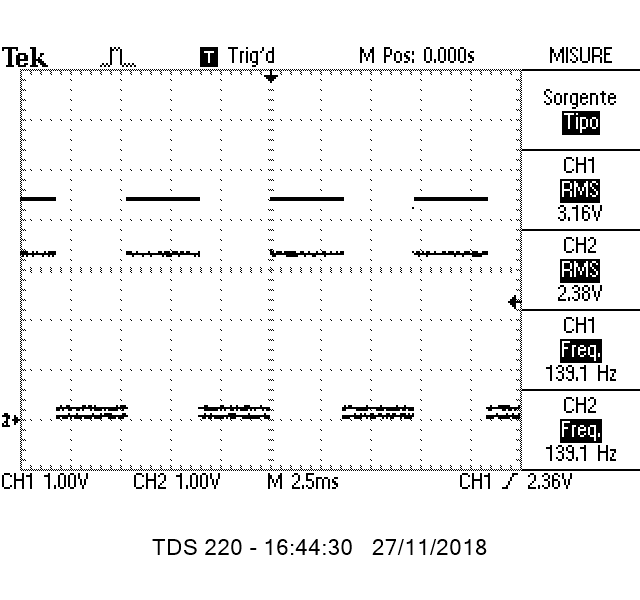
\includegraphics[width=\linewidth]{xor1.png}
	\captionof{figure}{Istantanea dell'oscilloscopio per il circuito XOR, ingresso $A=0$}
	\label{fig:XOR_A0}
	\end{center}
\end{Figure}

\begin{Figure}
	\begin{center}
	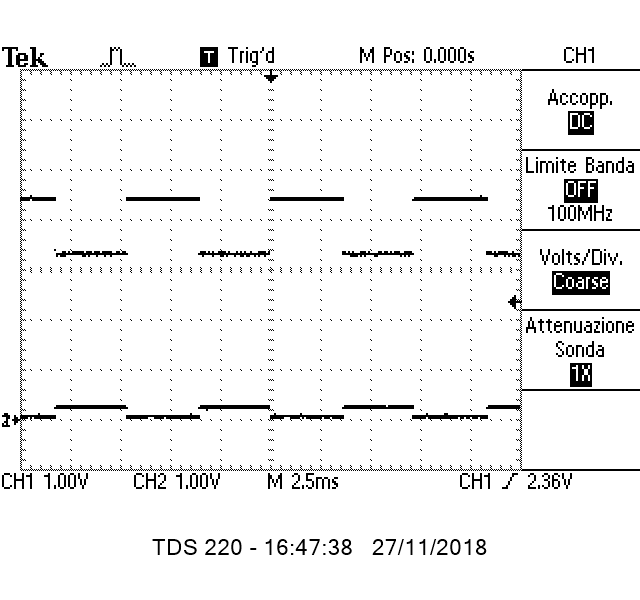
\includegraphics[width=\linewidth]{xor2.png}
	\captionof{figure}{Istantanea dell'oscilloscopio per il circuito XOR, ingresso $A=1$}
	\label{fig:XOR_A1}
	\end{center}
\end{Figure}


%==================================================
%             MULTIPLEXER A DUE INGRESSI
%==================================================
\section{Multiplexer a due ingressi}
Si realizza un circuito multiplexer a due ingressi, come da schema seguente.

%\begin{flushleft}
%\hspace*{-1cm}
%\begin{circuitikz}[scale=0.9]
%\draw (0,0) node[american nand port] (nand1) {}
%(2.2,1) node[american nand port] (nand2) {}
%(2.2,-1) node[american nand port] (nand3) {}
%(4,0) node[american nand port] (nand4) {}
%(nand1.in 1) to[short] (nand1.in 2)  
%(nand1.in 1 |- nand1.out) to [short,*-] (-3,0) to [short,*-*] (-2,0) 
%(-3,0) node[left]{$S$}
%(nand1.out) -| (nand3.in 1)
%(nand3.in 2) to[short, -*] ++(-3,0) node[left]{$A$}
%(nand2.in 1) to[short, -*] ++(-3,0) node[left]{$B$}
%(nand2.in 2) -| (-2,0)
%(nand3.out) -| (nand4.in 2)
%(nand2.out) -| (nand4.in 1)
%(nand4.out) to[R=$R$] ++(1,0) to[leDo] ++(0,-2) node[ground] {}
%;\end{circuitikz}
%\end{flushleft}

Il circuito implementa la funzione logica ridotta ai minimi termini
\[
Q = \overline{S}A + SB.
\]
L'ingresso di selezione $S$ permette di scegliere quale tra i livelli logici degli ingressi $A$ e $B$ riportare in uscita, in particolare, se $S = 0$ l'uscita sar� $Q = A$, al contrario, se $S = 1$, l'uscita sar� $Q = B$. Si riportano in Tabella~\ref{tab:multiplexer} i valori di tensione dell'uscita in corrispondenza delle diverse combinazioni dei livelli logici.

\begin{center}
\captionof{table}{Misure per il multiplexer}
\label{tab:multiplexer}
\begin{tabular}{c|c|c|c}
$S$ & $A$ & $B$ & $V_Q$ [\SI{}{mV}]  \\
 & & & ($\pm 0.5\%$) \\
\hline
0 & 0 & 0 & 56.6 \\
0 & 0 & 1 & 56.2 \\
0 & 1 & 0 & $4.07 \times 10^3$ \\
0 & 1 & 1 & $4.07 \times 10^3$ \\
1 & 0 & 0 & 56.85 \\
1 & 0 & 1 & $4.07 \times 10^3$ \\
1 & 1 & 0 & 56.6 \\
1 & 1 & 1 & $4.07 \times 10^3$ \\
\hline
\end{tabular}
\end{center}

Si connette il canale \texttt{CH1} dell'oscilloscopio all'ingresso $A$ e il canale \texttt{CH2} all'uscita $Q$; si pone l'ingresso di selezione $S=0$ e si invia all'ingresso $A$ un'onda quadra TTL mediante il generatore di segnali; l'ingresso $B$ � posto a $0$ logico. Si riporta in Figura~\ref{fig:multiplexerA} uno screenshot dell'oscilloscopio per questa configurazione, dal quale si evince che l'uscita riproduce l'ingresso. 

\begin{Figure}
	\begin{center}
	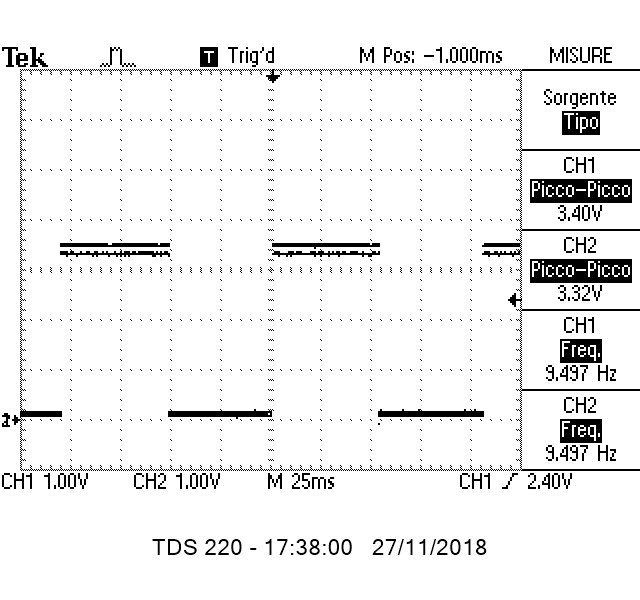
\includegraphics[width=\linewidth]{multiplexerTTLsuA.png}
	\captionof{figure}{Istantanea dell'oscilloscopio per il multiplexer, $S = 0$}
	\label{fig:multiplexerA}
	\end{center}
\end{Figure}

Si ripete l'esperimento ponendo $S=1$, $A=0$ e inviando all'ingresso $B$ un'onda quadra TTL. In questo caso il canale \texttt{CH1} dell'oscilloscopio � collegato all'ingresso $B$. Si riporta in Figura~\ref{fig:multiplexerB} l'istantanea dell'oscilloscopio per questa configurazione; si osserva anche qui la sovrapposizione tra segnale in ingresso e in uscita.

\begin{Figure}
	\begin{center}
	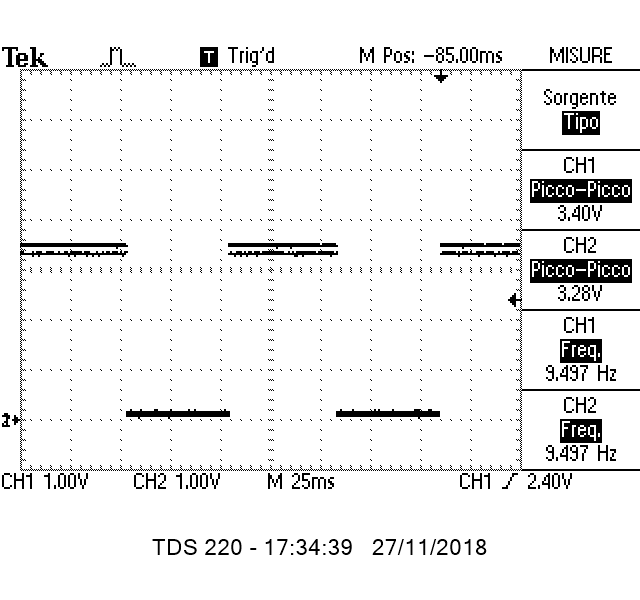
\includegraphics[width=\linewidth]{multiplexerTTLsuB.png}
	\captionof{figure}{Istantanea dell'oscilloscopio per il multiplexer, $S = 1$}
	\label{fig:multiplexerB}
	\end{center}
\end{Figure}

I segnali di ingresso e di uscita non si sovrappongono esattamente, ci� � dovuto al fatto che i livelli logici effettivi dell'integrato, misurati nella sezione precedente, differiscono dai valori di tensione tra cui oscilla l'onda quadra in ingresso.

Un'ulteriore verifica del circuito costruito pu� essere fatta ponendo l'ingresso $A$ a $0$ logico e inviando sull'ingresso $S$ e sull'ingresso $B$ due onde quadrate di frequenza rispettivamente $f_S$ e $f_B$, dove $f_S << f_B$. Un'istantanea dell'oscilloscopio in questa configurazione � riportata in Figura \ref{fig:multiplexer3}. Ci� che si vede � che l'onda quadra su $S$ fa commutare l'uscita tra il valore di $A$, che � nullo, e il valore di $B$, che � a sua volta un'onda quadra ma di frequenza pi� elevata rispetto a quella su $S$.

\begin{Figure}
	\begin{center}
	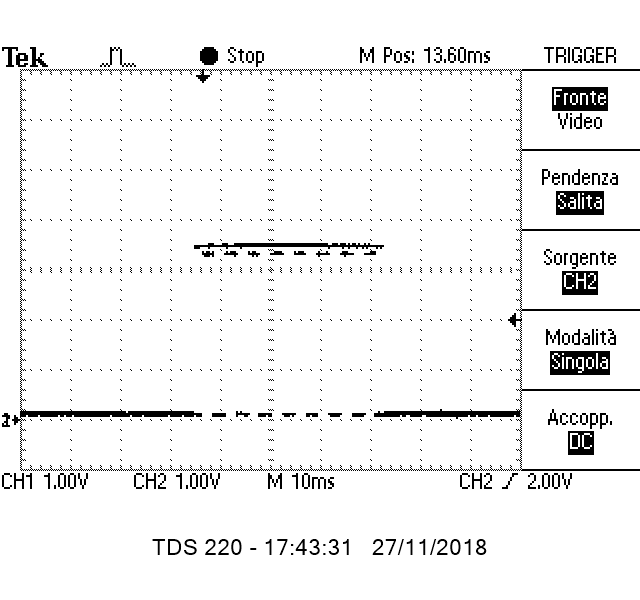
\includegraphics[width=\linewidth]{multiplexerBsu0QuadraSuAquadraSuSignal.png}
	\captionof{figure}{Istantanea dell'oscilloscopio per il multiplexer, $A = 0$ e si mandano su $S$ e $B$ due onde quadre con frequenza sul primo ingresso nettamente minore di quella sul secondo}
	\label{fig:multiplexer3}
	\end{center}
\end{Figure}

%==================================================
%             FLIP-FLOP S-R
%==================================================
\section{Flip-Flop Set-Reset}
Si realizza un \emph{flip-flop} S-R utilizzando tutte e 4 le porte NAND dell'integrato. La tavola della verit� � la seguente
\[
\begin{array}{cc|c}
S_n & R_n & Q_{n+1} \\
\hline
0 & 0 & Q_n \\
1 & 0 & 1 \\
0 & 1 & 0 \\
1 & 1 & ?
\end{array}
\]
e viene implementata dal circuito sotto illustrato. 

%\begin{circuitikz}[scale=0.9]
%\draw (0,1.6) node[american nand port] (nand1) {}
%(0,-1.6) node[american nand port] (nand2) {}
%(2,1) node[american nand port] (nand3) {}
%(2,-1) node[american nand port] (nand4) {}
%(nand1.in 1) to[short, -*] ++(-0.5,0) node[left] {$S$}
%(nand2.in 2) to[short, -*] ++(-0.5,0) node[left] {$R$}
%(nand1.in 2) -- (nand2.in 1) 
%(nand1.in 2) ++(0,-1.4) -- ++(-0.5,0) node[circ] {} node[left]{\texttt{CLK}}
%(nand1.out) -| (nand3.in 1)
%(nand2.out) -| (nand4.in 2)
%(nand3.in 2) -- ++(0,-0.5) node[](in1){}
%(nand4.in 1) -- ++(0,0.5) node[](in2){}
%(nand3.out) -- ++(0,-0.5) node[](out1){}
%(nand4.out) -- ++(0,0.5) node[](out2){}
%(in1) to[short] (out2)
%(in2) to[short] (out1)
%(nand3.out) to[R=$R_1$] ++(1,0) to[leDo] ++(2,0) node[](end){};
%\draw (nand4.out) to[R=$R_2$] ++(1,0) to[leDo] ++(2,0) node[ground](ground) {}
%(end) to[short] (ground)
%;\end{circuitikz}

Si utilizzando dei LED per verificare il corretto funzionamento del circuito, protetti verso massa dalle resistenze $R_1 = \SI{111 \pm 111}{\kilo\ohm}$ e $R_2 = \SI{111 \pm 111}{\kilo\ohm}$. Inizialmente si fornisce un impulso di clock manuale all'ingresso \texttt{CLK} mediante il generatore di tensione, utilizzando un ingresso statico con resistenza di pull-up e interruttore verso terra, come gi� descritto precedentemente. Si controlla dunque che il circuito si comporti come previsto, impostando alternativamente $S=1$, $R=0$ o $S=0$, $R=1$, azionando il clock e osservando il valore logico dell'uscita mediante un multimetro. Si riportano in Tabella~\ref{tab:flip-flop_controllo} i valori di tensione e i corrispondenti valori logici per le diverse configurazioni, ordinati temporalmente (secondo l'indice $n$).

\begin{center}
\captionof{table}{Misure per il controllo del flip-flop}
\label{tab:flip-flop_controllo}
\begin{tabular}{c|c|c|c}
n & $V_S$ [\SI{}{V}] & $V_R$ [\SI{}{V}] & $V_Q$ [\SI{}{V}] \\
\hline
1 & $2.3 \times 10^{-3}$ & $1.26\times 10^{-3}$ & $67.5 \times 10^{-3}$ \\
2 & $5.0$ & $1.70\times 10^{-3}$ & $3.21$ \\
3 & $2.0 \times 10^{-3}$ & $5.0$ & $67.1 \times 10^{-3}$ \\
\hline
\end{tabular}
\end{center}

Le misure servono per evidenziare la memoria del circuito: quando entrambi gli ingressi sono sullo zero logico la misura di output dipende dalla storia precedente, ossia dal valore di output prima che gli ingressi fossero messi a zero.

Si connette quindi il segnale di set $S$ al \texttt{CH1} dell'oscilloscopio e l'uscita $Q$ al canale \texttt{CH2}. Si pone $R=0$, il clock $\texttt{CLK} = 1$ e si invia all'ingresso $S$ un'onda quadra TTL. Si riporta in Figura~\ref{fig:flip-flop1} un'istantanea dell'oscilloscopio per questa configurazione, e si osserva che l'uscita � costante e pari al livello logico $1$ in quanto i settaggi successivi al primo non influiscono sullo stato del flip-flop, come previsto dalla tavola della verit�. 

\begin{Figure}
	\begin{center}
	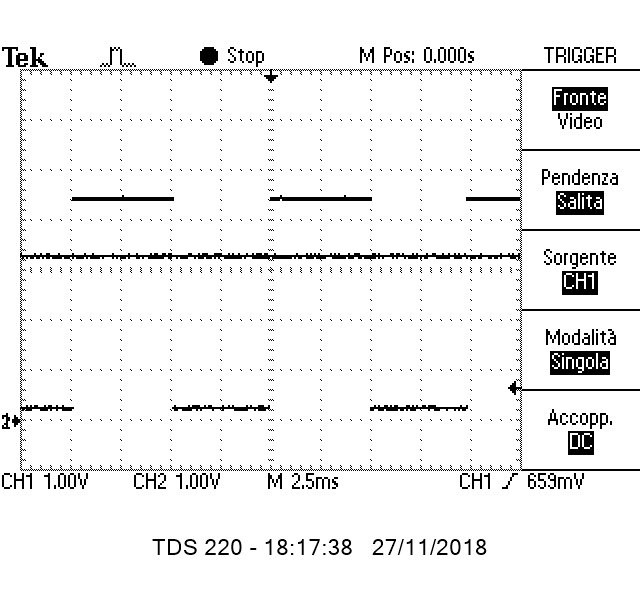
\includegraphics[width=\linewidth]{FlipFlopTTLset.png}
	\captionof{figure}{Istantanea dell'oscilloscopio per il flip-flop, onda quadra TTL su $S$ e $\texttt{CLK} = 1$}
	\label{fig:flip-flop1}
	\end{center}
\end{Figure}

Analogamente ponendo $S=0$ e inviando all'ingresso $R$ un'onda quadra TTL si osserva un'uscita costante sullo zero logico, come osservabile in Figura \ref{fig:flip-flop2}

\begin{Figure}
	\begin{center}
	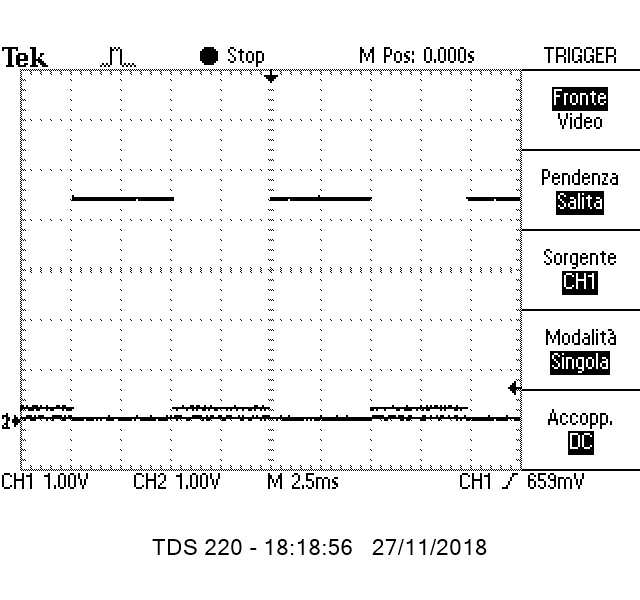
\includegraphics[width=\linewidth]{FlipFlopTTLreset.png}
	\captionof{figure}{Istantanea dell'oscilloscopio per il flip-flop, onda quadra TTL su $R$ e $\texttt{CLK} = 1$}
	\label{fig:flip-flop2}
	\end{center}
\end{Figure}




\end{multicols}

\newpage
\section{Appendice}
\begin{center}
\captionof{table}{Misure per il livello di commutazione delle porte logiche TTL}
\label{tab:commutazione}
\begin{tabular}{c|c}
\hline
   $V_{i}$ [V] &   $V_{o}$ [V] \\
\hline
         0.012 &         3.780 \\
         0.034 &         3.760 \\
         0.053 &         3.740 \\
         0.071 &         3.722 \\
         0.116 &         3.676 \\
         0.150 &         3.643 \\
         0.175 &         3.616 \\
         0.199 &         3.593 \\
         0.215 &         3.577 \\
         0.234 &         3.560 \\
         0.286 &         3.500 \\
         0.328 &         3.460 \\
         0.403 &         3.370 \\
         0.540 &         3.100 \\
         0.647 &         2.800 \\
         0.762 &         2.320 \\
         0.850 &         1.350 \\
         0.903 &         0.400 \\
         0.927 &         0.122 \\
         1.100 &         0.059 \\
         1.330 &         0.059 \\
         1.530 &         0.059 \\
         1.990 &         0.059 \\
         2.360 &         0.059 \\
         2.780 &         0.059 \\
         3.240 &         0.059 \\
         3.580 &         0.059 \\
         3.860 &         0.059 \\
         4.200 &         0.059 \\
\hline
\end{tabular}
\end{center}


\bibliography{bib}
\bibliographystyle{ieeetr}



%ESEMPIO DI FIGURA
%\begin{Figure}
%	\begin{center}
%	\includegraphics[width=\linewidth]{comune.png}
%	\captionof{figure}{Istantanea dell'oscilloscopio per l'amplificatore differenziale, misura di $A_c$}
%	\label{fig:Ac_differenziale}
%	\end{center}
%\end{Figure}


%ESEMPIO DI TABELLA
%\begin{center}
%\captionof{table}{Misure per la stima di $A_c$}
%\label{tab:Ac_differenziale}
%\begin{tabular}{c|c|c|c}
%$f$ [\SI{}{Hz}] & $V_i$ [\SI{}{V}] & $v_o$ [\SI{}{mV}] & $A_c = v_o / V_i$ \\
%\hline
%      149.5 &        3.90 &         11.3 & 2.90e-03 \\
%      222.0 &        3.90 &         11.5 & 2.95e-03 \\
%      281.0 &        3.90 &         11.8 & 3.03e-03 \\
%      359.0 &        3.90 &         11.8 & 3.03e-03 \\
%      461.0 &        3.90 &         12.2 & 3.13e-03 \\
%\hline
%\end{tabular}
%\end{center}
\end{document}